\chapter{Troubleshooting}\label{ch:troubleshooting}
\section{Boot Order} \label{sec:BootOrder}
The communications protocols between the USRP and the host follows the PCIe standard. It is essential that the drivers are loaded up during boot up. It is highly advised against hot swapping or unplugging PCIe cables while the host is booted up and running. Secondly care must be taken while booting up the system by following the sequence recommended by NI in order to avoid synchronisation issues.

\begin{enumerate}
    \item Connect the PCIe cables from the PCIe port of the USRPs to the PCIe cards mounted on the Host (section \ref{ssec:PCIe-8371})
    \item Power up the USRPs once the above step has been completed
    \item Power up the PC and wait for the device to boot up
    \item Check the NI MAX (NI's software for managing NI devices) Software to see if the devices have been recognised by the PC
    \item When all the USRPs appear on the NI MAX they are ready to be used
\end{enumerate}

\section{Synchronisation of the USRPs} \label{sec:USRPSync}

USRPs are complex devices which combine analog tranceivers and digital Xilinx Kintex-7 FPGA, which does all the compute intensive tasks. Figure \ref{fig:USRPInternals} shows a block diagram of a \textbf{single} RF channel with the internal components of the USRP. There are two such channels in a given USRP 2940.

The figure shows that a single RF channel can be used either as a single antenna transmitter (\textbf{TX1}) or a single antenna receiver (\textbf{RX1/RX2}). RX1 and RX2 \textbf{cannot} be used simultaneously.

The 2 radio channels within a USRP are either synchronised using the REF IN signal which is a 10 MHz supplied by an external clock distributer (section \ref{ssec:CDA-2990}) or by using the internal 10MHz oscillator. They share the same reference clock for all the PLLs and the VCOs as illustrated in figure \ref{fig:USRPInternals}. It was inferred from tests that the RF path delay for the Low Noise Amplifiers (LNA) are not matched between the channels in the USRP and therefore leading to phase shifts between the 2 RF channels on the single USRP. This results in unsynchronous transmit and receive data between the channels which is not the preffered mode of operation for a MIMO setup as receive and transmit synchronisation is key. Furthermore the delay is not a constant for every new run of the system, rather its a new delay for every rerun. This is the limitation of the hardware and caused by delays in the RF analog path. The delay does remain constant within the duration of a run.

The Octoclock provides a common 10 MHz sampling clock which all the USRPs synchronize to. The Octoclock also has a PPS Trigger which is a pulse per second trigger which is used as a sampling trigger for different USRPs.

\begin{figure}[h]
    \centering
    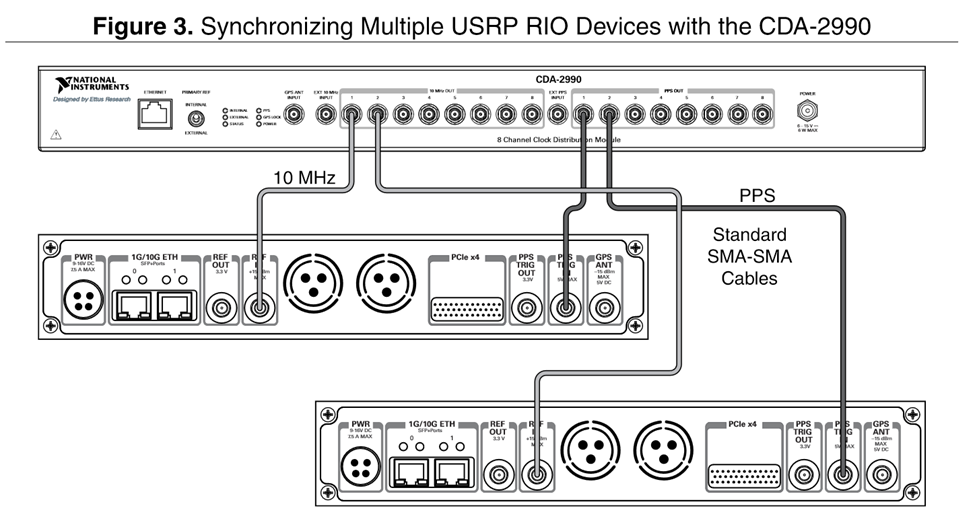
\includegraphics[width=\linewidth]{images/USRPHWConnections.png}
    \caption{The connections from the Octoclock to the USRP}
    \label{fig:OctoUSRPConnections}%
\end{figure}

\begin{landscape}% Landscape page
    \begin{figure}[H]
        \centering
        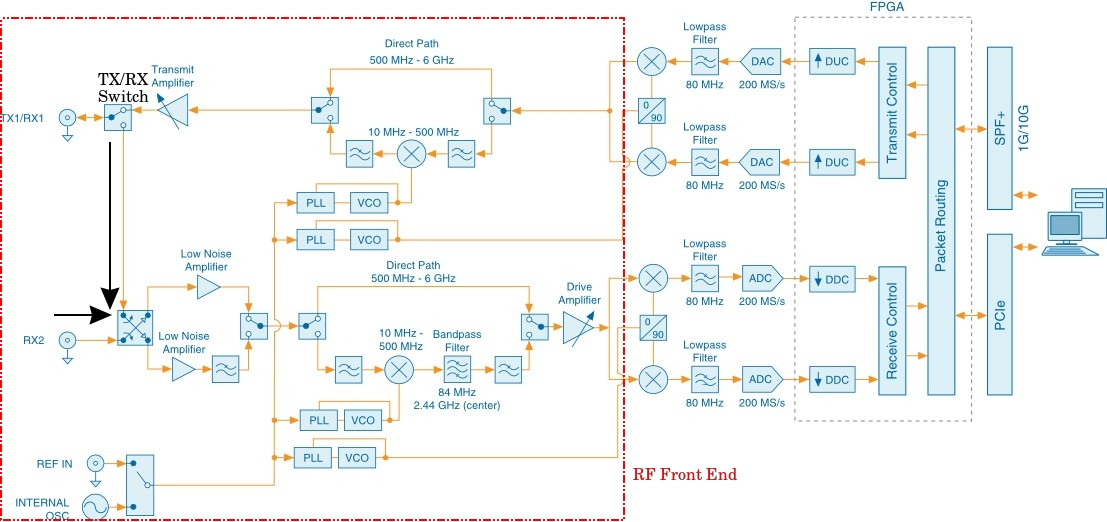
\includegraphics[width=\linewidth]{images/USRPInternalsEdited.jpeg}
        \caption{USRP 2940 Internal Components}%
        \label{fig:USRPInternals}%
    \end{figure}
\end{landscape}

The following section describes the test setup used to verify the functional specification of the Octoclock. Figure \ref{fig:RefSigFFT} show the REF IN coming in from 2 different ports of the octoclock each terminated with a 50 Ohm resistor and measured with an oscilloscope. The experiment was carried out to verify the synchronicity of the reference clocks from two different ports of the octoclock. The FFT of the signal also shows that the tone lies at 10 MHz.

\begin{figure}[h]
    \centering
    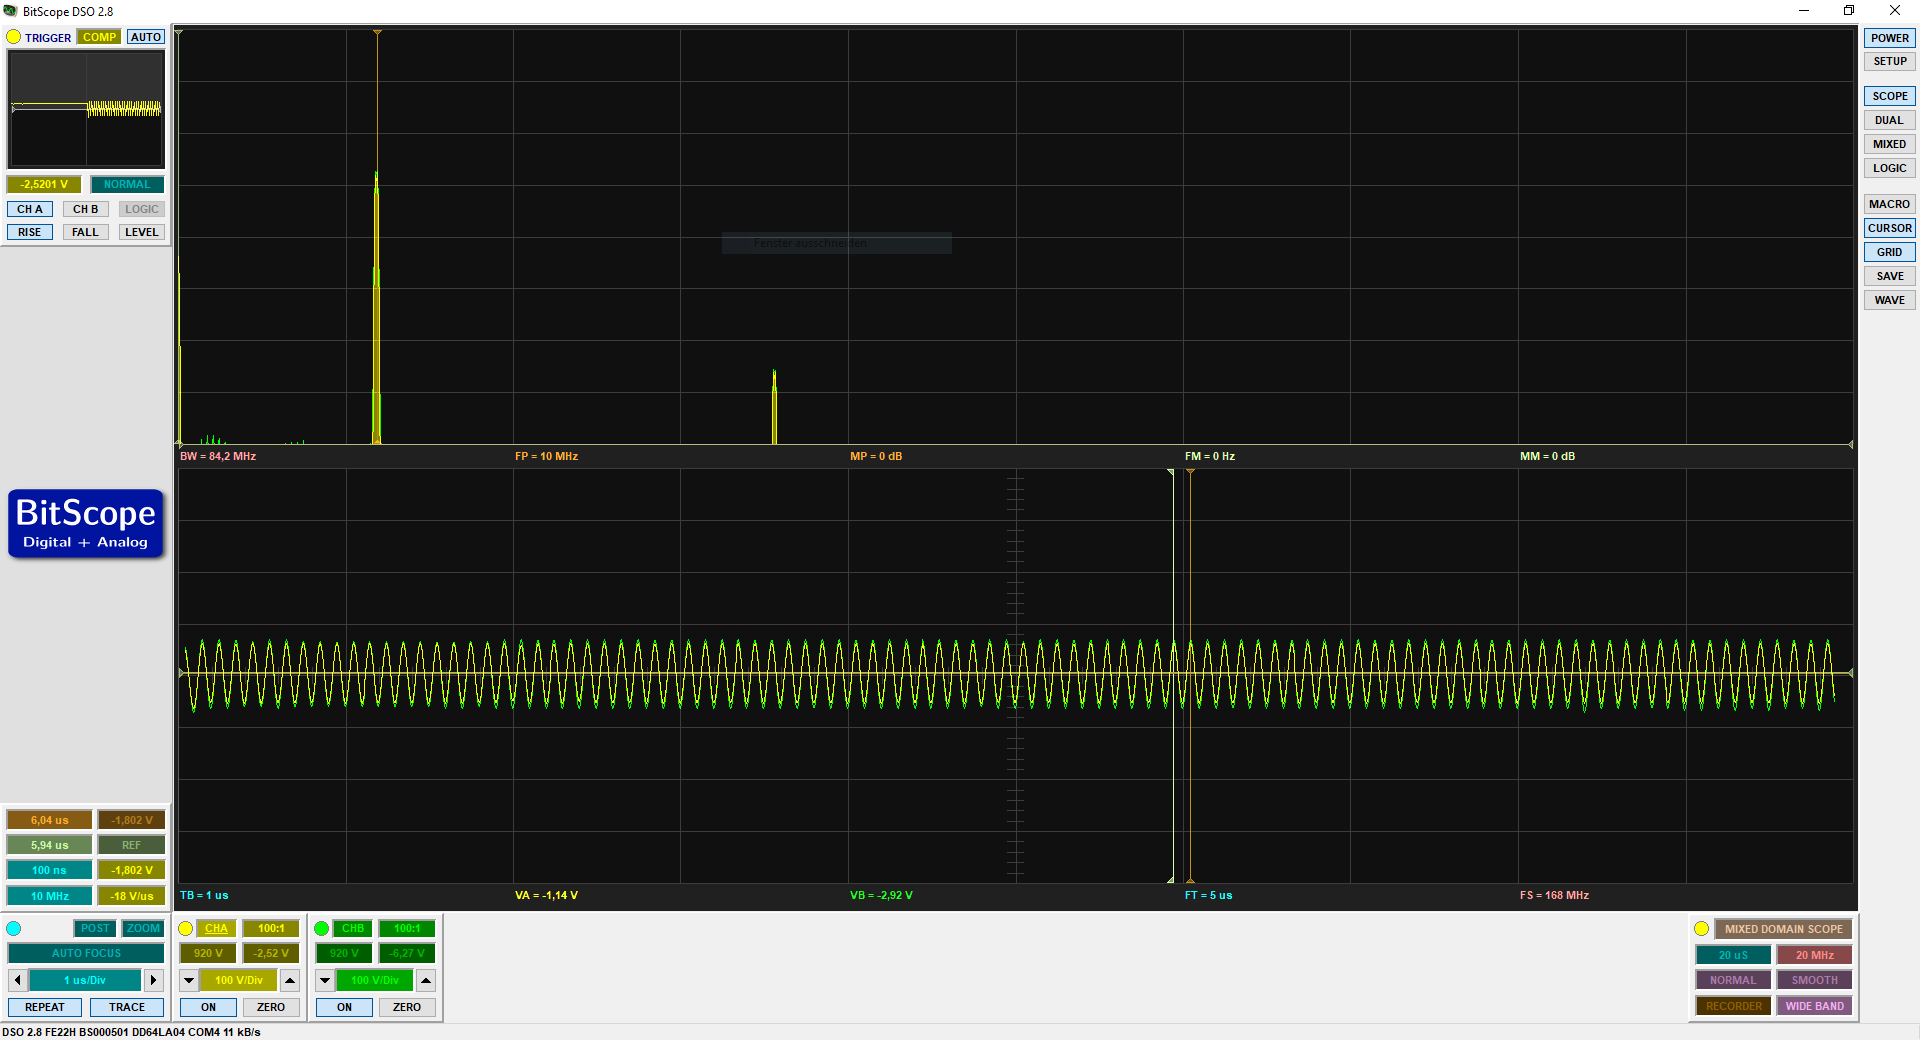
\includegraphics[width=\linewidth]{images/PPSTrigFFT.png}
    \caption{The 10 MHz REF IN clock as seen at the output of two respective channels of the Octoclock. The yellow is from ch1 and the green is from channel 2 which are connected to USRP1 and USRP2 respectively. The top half is the Fourier transform and the bottom half is the time domain signal}
    \label{fig:RefSigFFT}%
\end{figure}

Figures \ref{fig:PPSTrig} and \ref{fig:PPSTrigZoomedIn} show 2 PPS (Pulse per Second) triggers received from 2 ports of the octoclock each terminated with a 50 Ohm resistor and measured using an oscilloscope. The signals found to be aligned and have a rising edge every second as we expect.

It can be inferred from the design of the Octoclock \ref{ch:HWSchOctoClock} that the REF IN is internally generated by the Octoclock and distributed among all the ports. Alternatively there is an option to feed the an external reference input to the octoclock and distribute this reference among the other ports.

\begin{figure}[H]
    \centering
    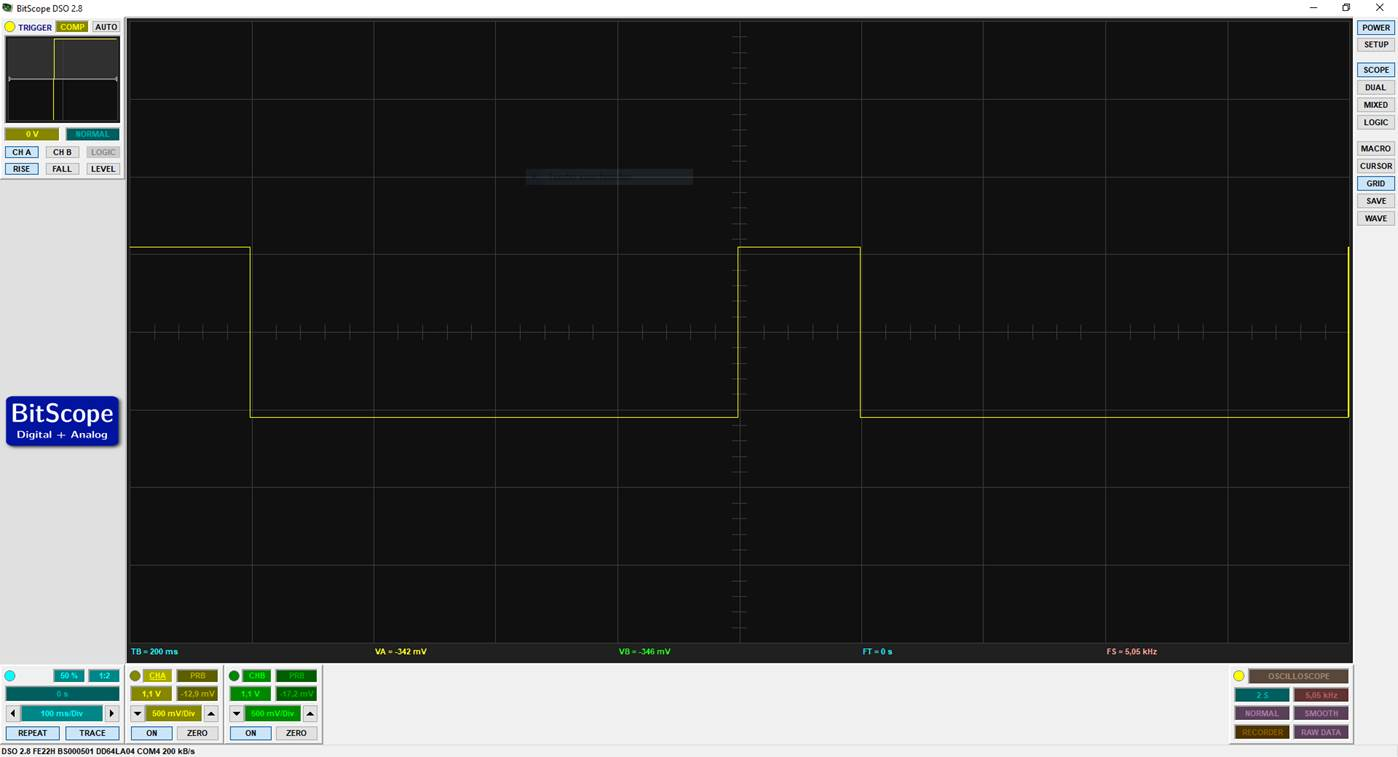
\includegraphics[width=\linewidth]{images/PPSTrig.jpg}
    \caption{Figure shows a zoomed-out view of the PPS Trig Out which occurs every 1s and the high pulse is 200ms long.}
    \label{fig:PPSTrig}%
\end{figure}

\begin{figure}[htb]
    \centering
    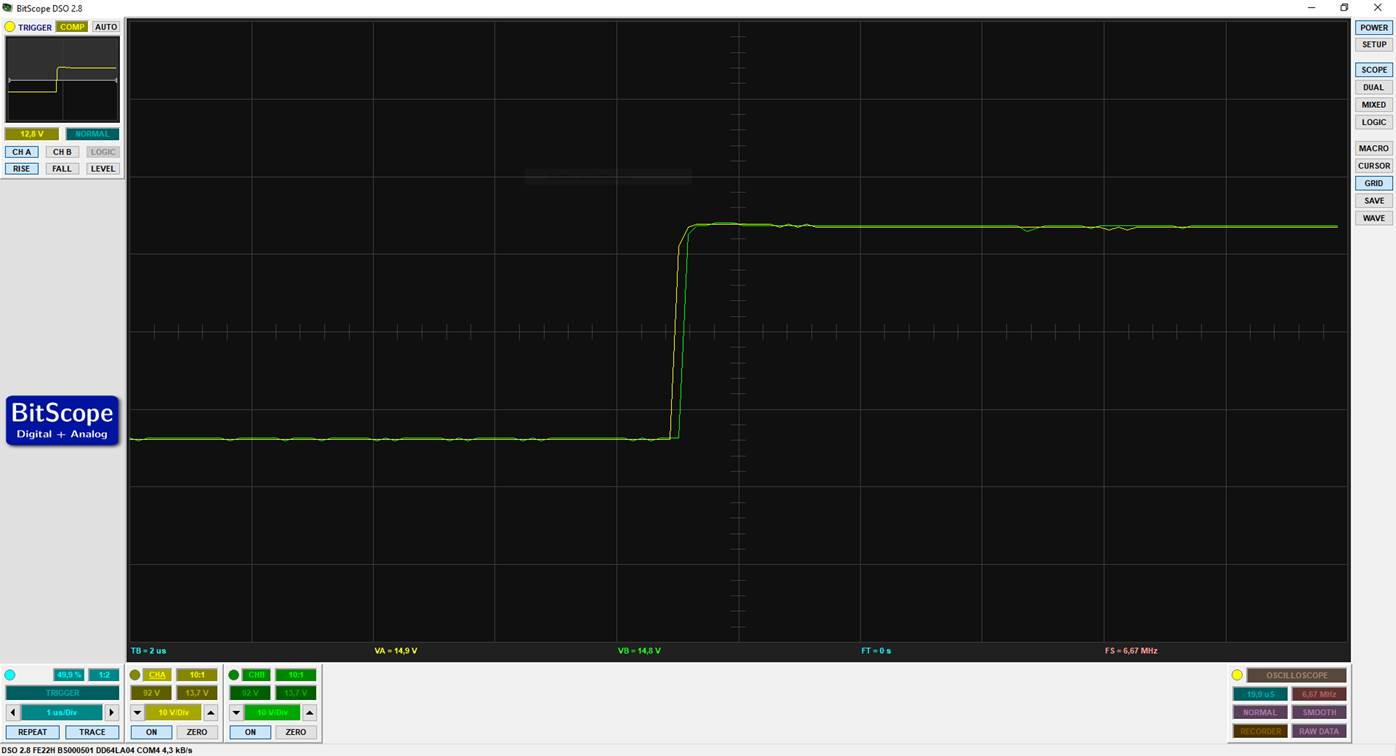
\includegraphics[width=\linewidth]{images/PPSTrigZoomIn.jpg}
    \caption{Figure shows the PPS trigger signal from the Octoclock. The slight shift is potentially an artifact from the measurement instrument as the bandwidth of the measurement tool was limited (20MHz).}
    \label{fig:PPSTrigZoomedIn}%
\end{figure}

Finally after verifying the Octoclock functionality, a test was devised to measure the synchronisity of the Tranceiver. For this 2 USRP devices were connected as shown in \ref{fig:OctoUSRPConnections} and tests were run in loopback mode where the TX1 of each RF channel was connected to the respective RX2 of the same RF channel. A pure tone is sent as IQ samples from each TX1 port of each USRP 1 and USRP 2. This test was conducted by using 1m 50 Ohm cables to eliminate the air interface. Matched length cables avoid phase delays and are critical in this measurements.

The function sent at the transmitter side is described as follows

\begin{equation}
    y(t) = cos(\omega{t}) + j*sin(\omega{t})
\end{equation}
where the I Signal is $cos(\omega{t}$) and the Q Signal is $sin(\omega{t}$).

Ideally the same signal should be received on all RX ports, where as the signals are received with a relative random phase shift. Figure \ref{fig:SyncFail2Ch} below shows the results of the tests showing the phase difference when one USRP transmits the same sine tone on the 2 respective TX1 channels of the 2 USRPs, while the signals are received on the respective RX2 channels of each RF channel.

\begin{landscape}
\begin{figure}[H]
    \centering
    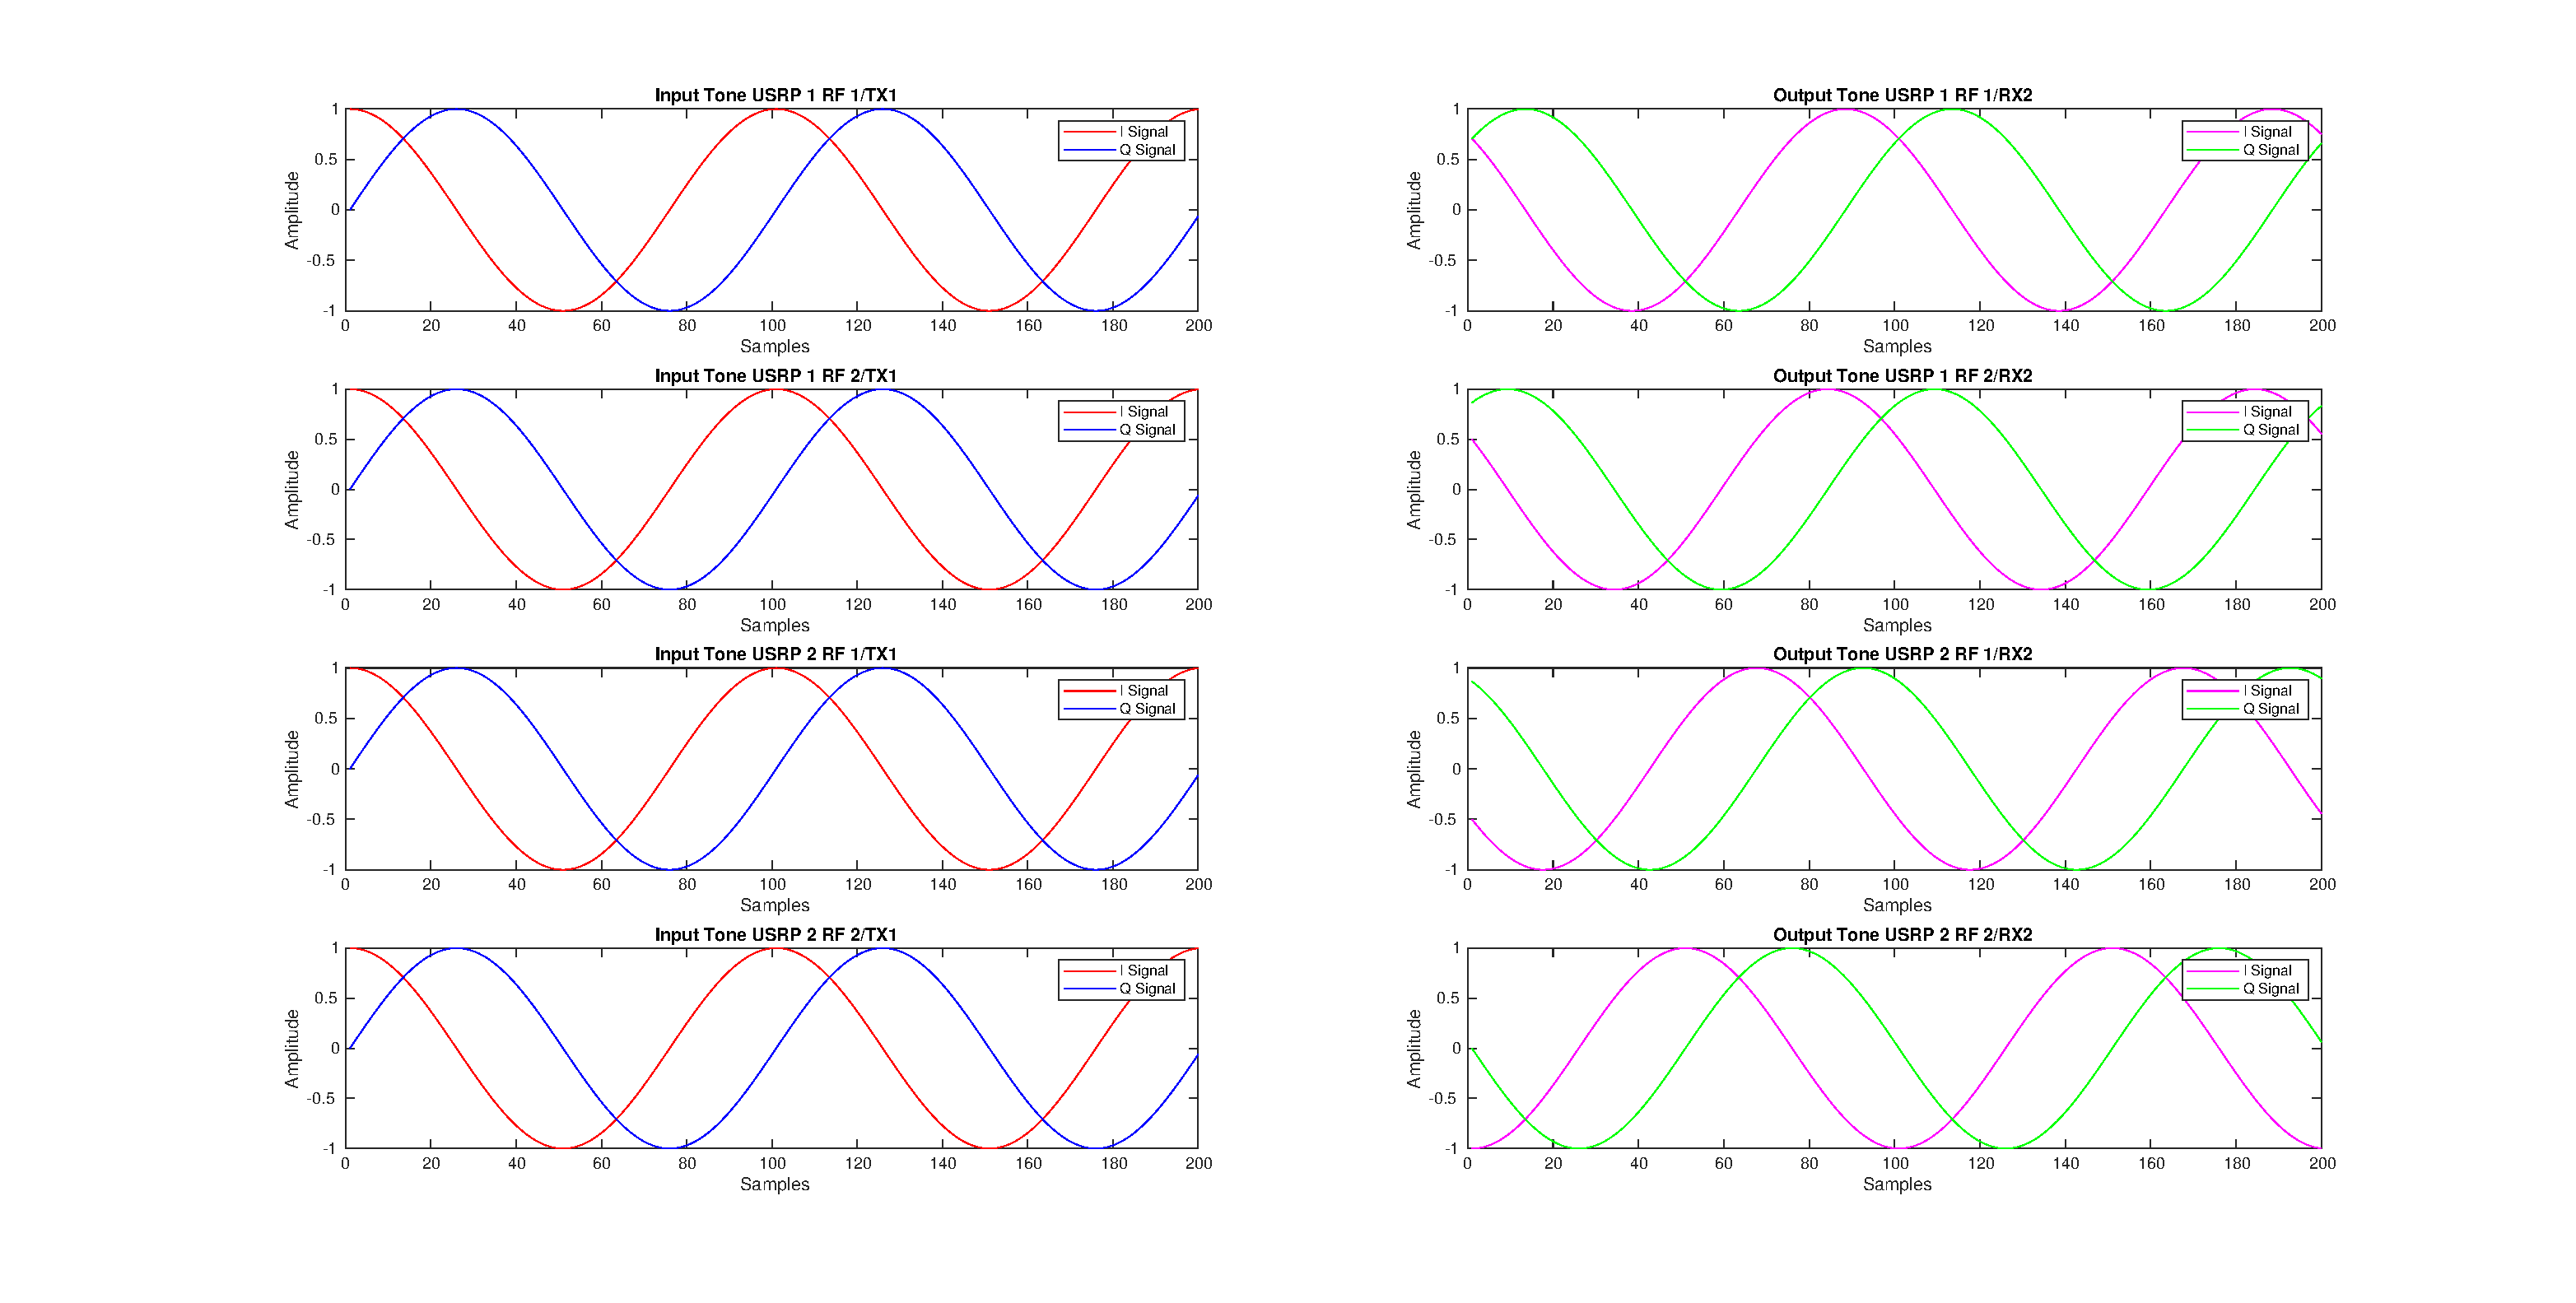
\includegraphics[width=22cm]{images/SyncIssues.eps}
    \caption{The left waveforms are the TX waveforms and the right waveforms are the RX waveforms. It can be seen that the received IQ waveforms are unsynchronised and clearly have a phase shift}
    \label{fig:SyncFail2Ch}%
\end{figure}
\end{landscape}

\chapter{Schematic Octoclock}
\label{ch:HWSchOctoClock}

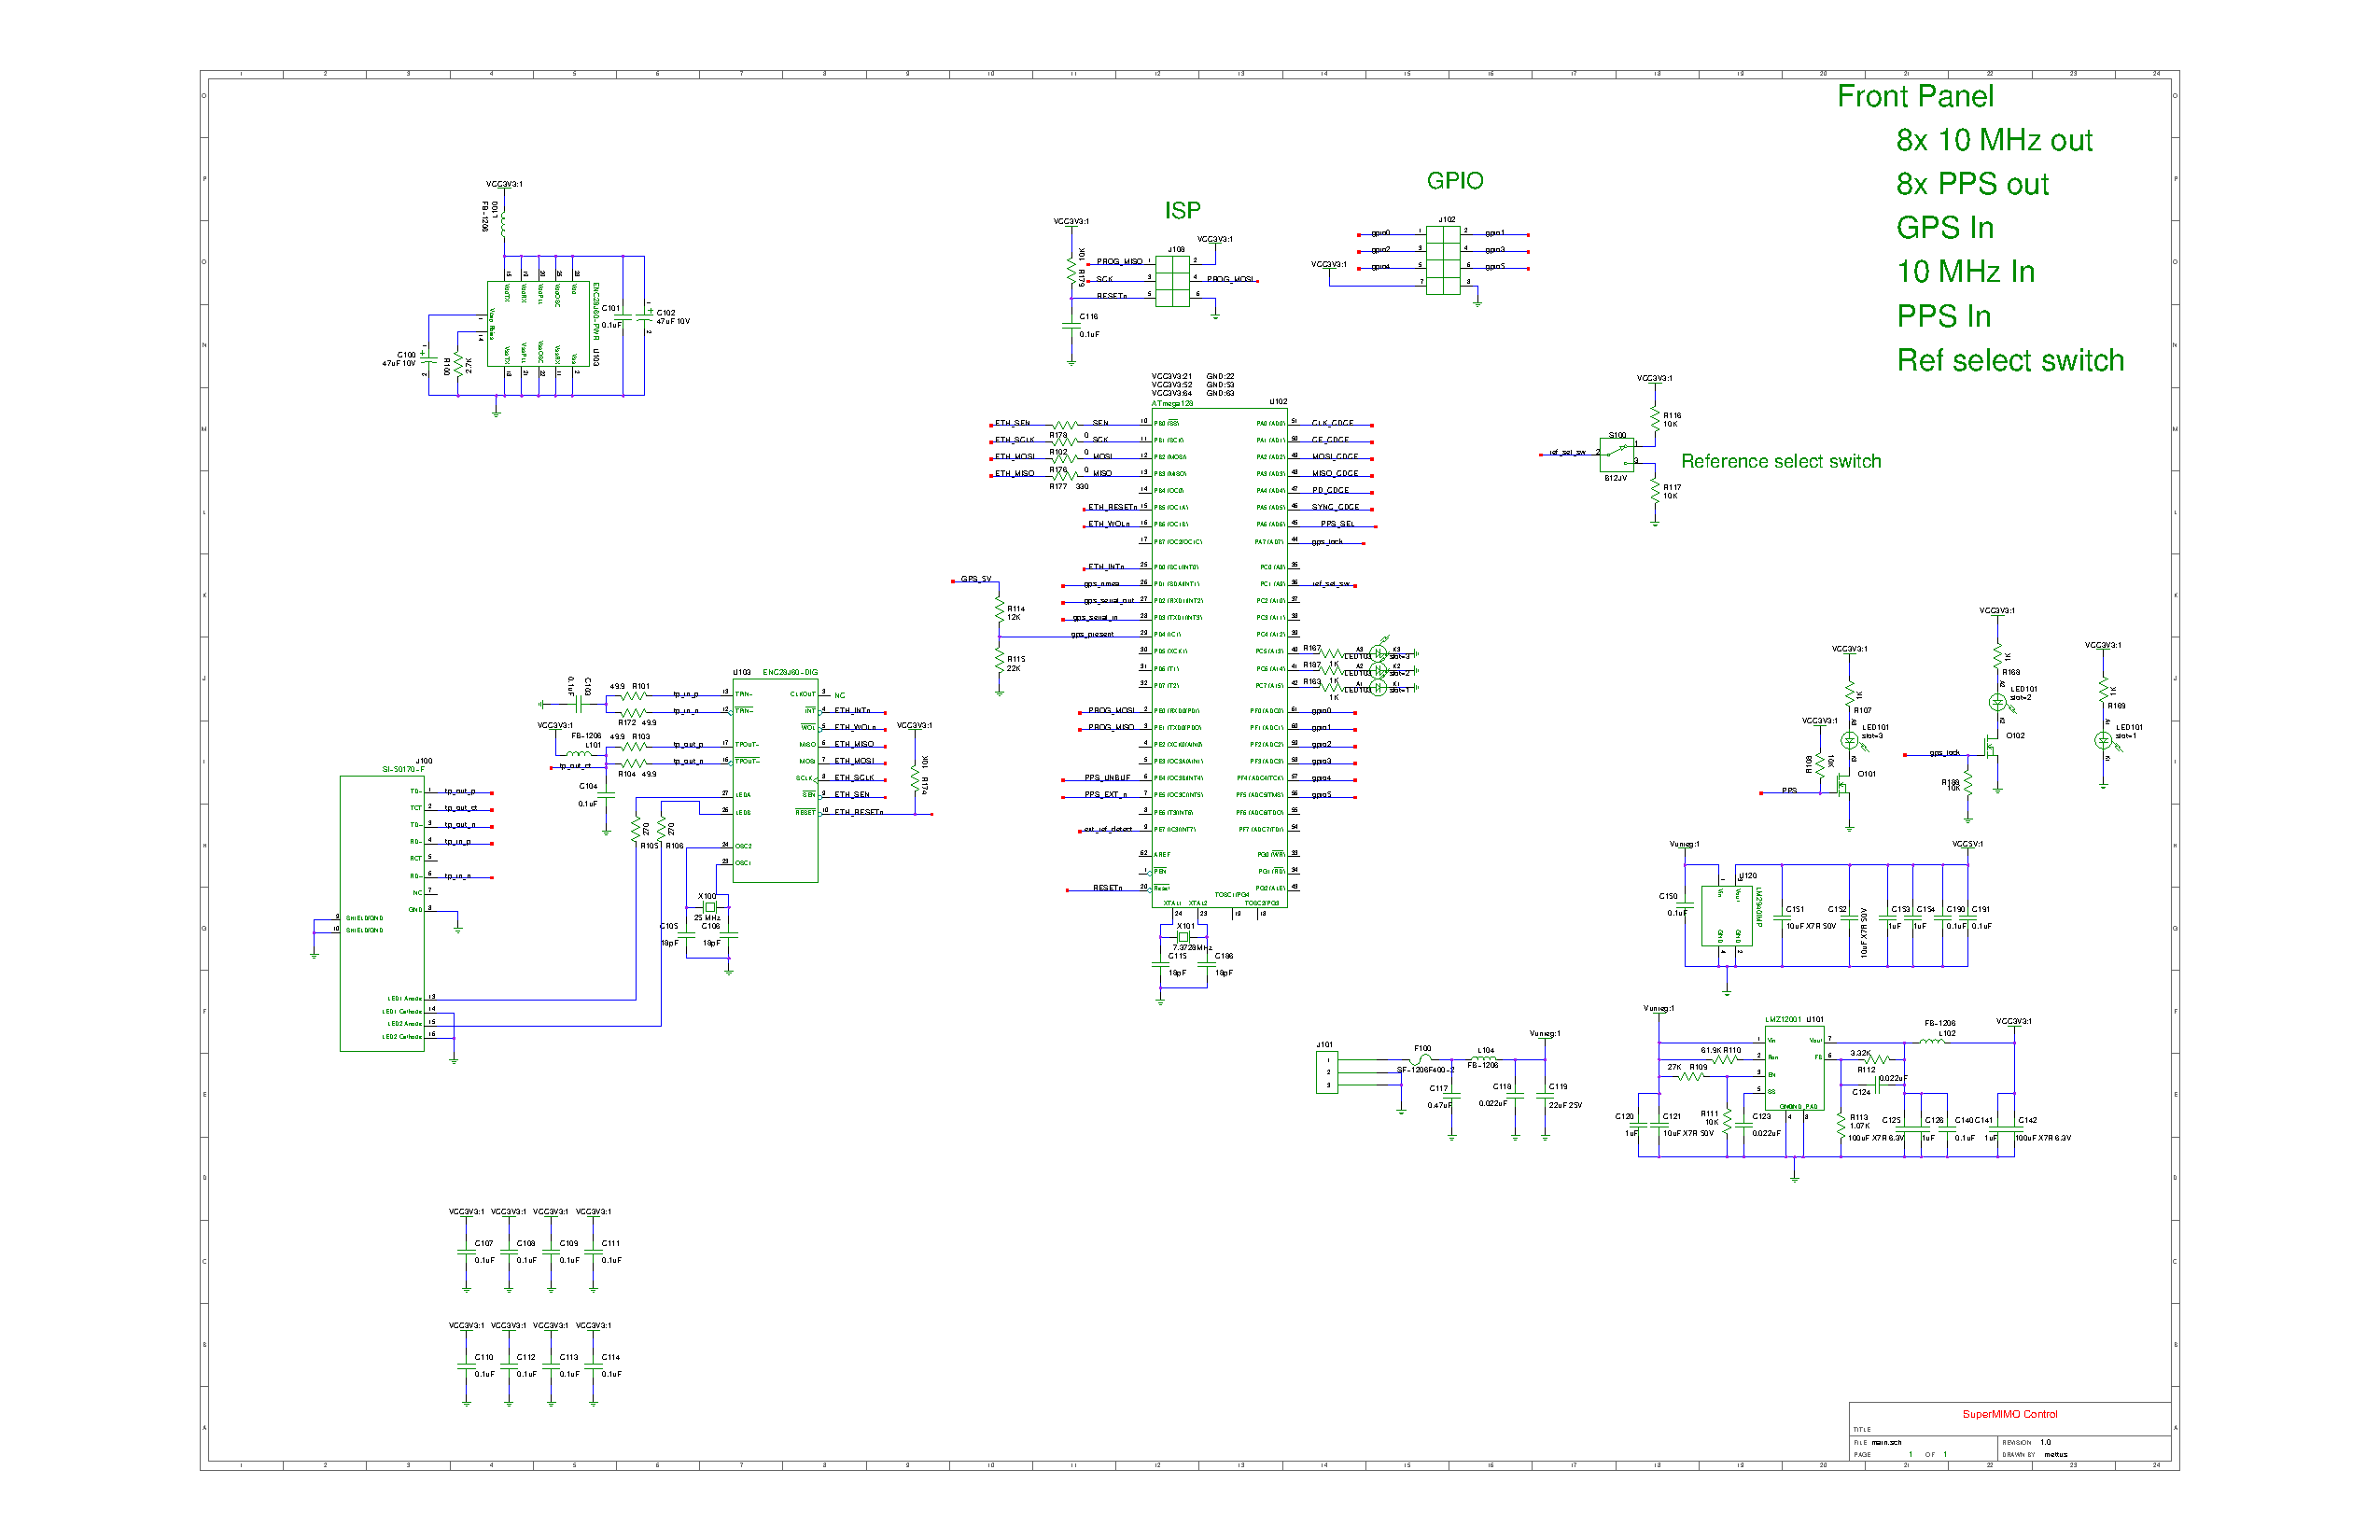
\includepdf[pages={1,2}, angle=-90]{images/OctoclockSchematics/octoclock.pdf}
